\begin{exo}{}
	Compléter le schéma ci-dessous en associant à chaque zone le symbole de l'ensemble de nombres qui convient.

	\begin{center}
		\begin{tikzpicture}[scale=0.8, every node/.style={scale=0.9}]
			\draw[thick, fill=blue!5] (0,0) ellipse (4.5cm and 3.3cm);
			\draw[thick, fill=green!8!white] (-0.3,0) ellipse (3.4cm and 2.6cm);
			\draw[thick, fill=orange!12!white] (-0.6,0) ellipse (2.4cm and 2.1cm);
			\draw[thick, fill=purple!10!white] (-0.9,0) ellipse (1.5cm and 1.5cm);
			\draw[thick, fill=gray!20!white] (-1.2,0) ellipse (0.7cm and 1.0cm);
			\node[fill=white, inner sep=6pt, scale=0.8] at (-1.2,0) {\ \dots\ };
			\node[fill=white, inner sep=6pt, scale=0.8] at (0,0) {\ \dots\ };
			\node[fill=white, inner sep=6pt, scale=0.8] at (1.1,0) {\ \dots\ };
			\node[fill=white, inner sep=6pt, scale=0.8] at (2.3,0) {\ \dots\ };
			\node[fill=white, inner sep=6pt, scale=0.8] at (3.7,0) {\ \dots\ };
			\node[scale=1.2, black] at (-1.2,-0.7) {$7$};
			\node[scale=1.2, black] at (-0.3,0.65) {$-3$};
			\node[scale=1.2, black] at (0.9,-0.9) {$-0,5$};
			\node[scale=1.2, black] at (2.0,1.2) {$\dfrac{2}{3}$};
			\node[scale=1.2, black] at (3.2,-1.4) {$\sqrt{2}$};
		\end{tikzpicture}
	\end{center}
\end{exo}
